\chapter{拥塞博弈}

\makeatletter
% 核心步骤 A：解除公式与 section 的绑定
% 如果发现公式还在随 section 重置，强制解除它
\@removefromreset{equation}{section}
\@removefromreset{figure}{section}
\@removefromreset{table}{section}

% 核心步骤 B：确保它们只随 chapter 重置
\@addtoreset{equation}{chapter}

% 核心步骤 C：统一编号格式 (章.序号)
\renewcommand{\theequation}{\thechapter.\arabic{equation}}

\makeatother



拥塞是指使用共享资源(如道路)的人越多，该资源的使用成本(cost)越高。在拥塞博弈(congestion game)中，玩家需要决定使用哪些资源，目标是最小化自己的成本。这种相互作用之所以构成一个博弈，是因为每个玩家的成本也取决于其他玩家的选择。

我们把拥塞网络(congestion network)作为交通模型来研究。在这个模型中，每个用户都要从起点到终点选择一条路线。网络中的每条边都可能产生拥塞，并且使用该边的人数越多，每个用户承担的成本就不会下降。本章的核心结果(定理~\ref{theo:2.2})表明，每个拥塞博弈都存在一个均衡(equilibrium)；在该均衡下，没有任何单个用户能仅靠改换路线来降低自己的成本。

与第 1 章类似，本章也是对博弈论中一个活跃而丰富的领域作入门介绍。我们会很快看到一些重要且并不平凡的结果。同时，在进入一般理论之前，本章也会引入博弈论中的策略和均衡概念。

均衡是用户为了最小化自身成本而进行自私路由的结果。这一结果通常并不是社会最优(social optimum)的，因为社会最优方案可能具有更低的平均成本。一个简单例子是“庇古网络”(Pigou network，见第 \ref{sec-2.2} 节)，它以英国经济学家亚瑟·庇古命名；庇古曾将外部性(如拥塞)的概念引入经济学。更令人惊讶的是，著名的布雷斯悖论(Braess paradox，见第 \ref{sec-2.3} 节)表明，增加道路网络的容量反而可能加剧均衡状态下的拥塞。

在第 \ref{sec-2.4} 节中，我们给出拥塞网络的一般定义；在第 \ref{sec-2.5} 节中，我们证明每个拥塞博弈都存在均衡。证明的关键是一个精心构造的势函数(potential function)。它虽然只是一个单一函数，却能同时反映每个用户改变策略时自身成本的变化。因此，这个势函数在所有策略组合上的最小值就定义了一个均衡。

在第 \ref{sec-2.6} 节中，我们解释这个模型的更广泛背景。本章采用的是原子流(不可拆分流)(atomic, non-splittable flow)的离散模型，其中有限数量的单个用户分别选择自己的出行路线。正如后面的例子所示，当“最后一个”用户可以在多条边之间同样最优地选择时，均衡往往不是唯一的。若用户数量趋于无穷，则得到可拆分流(splittable flow)的连续模型；在这个模型中，一个用户可以被看作从起点前往终点的“用户群体”中的无穷小部分。此时均衡通常是唯一的，但其存在性证明更具技术性，本章不展开。

我们还会提到无政府代价(Price of Anarchy)，它用于比较最差均衡成本与社会最优成本。更多细节可参考第 \ref{sec-2.7} 节中的文献说明。

\section{预备知识和学习目标}

本章不需要特别的预备知识。我们会使用有向图(digraph)的基本术语，例如节点(node)、边(edge)以及连接同一对节点的多条“平行”边(parallel edges)；这些概念会在第 \ref{sec-2.4} 节中正式定义。少量地方会用到标准微积分，用来求单变量函数的最小值。在第 \ref{sec-2.5} 节中，网络中的流(flow)由各条边 \(e\) 上的流量 \({f}_{e}\) 组成，并统一记为 \(f\)。

学习本章后，你应该能够:

\begin{itemize}
\item 理解拥塞网络和成本函数的含义，以及用户选择路径后如何在网络边上形成流量；
\item 求出网络中的均衡流和社会最优流，并比较二者的差异；
\item 理解势函数为什么能够用来寻找均衡。
\end{itemize}

\section{引言:庇古网络}\label{sec-2.2}

高峰时段出行往往比平时耗时得多。通勤者乘公交车时可能需要排队上车，公交车多了会挤占公交专用道，汽车也会造成拥堵；每个绿灯周期能够通过的车辆数毕竟有限。人们可以选择公交、步行或骑自行车，开车的人也可以选择不同路线。拥堵使出行变慢，而拥堵程度又取决于有多少人选择了同一种交通方式或同一条路线。我们假设每个人都会尽量选择对自己最好的路线，但哪条路线最好又取决于其他人的选择。这种相互影响正是一个博弈。下面我们建立一个数学模型，精确定义这个博弈的规则。

图~\ref{fig:2.1}给出了一个简单的拥塞网络。这个网络只有两个节点：起点 \(o\) 和终点 \(d\)，以及两条从 \(o\) 指向 \(d\) 的边。假设有若干用户都想从 \(o\) 到 \(d\)，每个用户可以任选其中一条边。每条边都有一个成本函数 \(c\left( x\right)\)，表示当这条边上有 \(x\) 个用户，也就是负载为 \(x\) 时，每个使用者需要承担的成本。上边的成本恒为 \(c\left( x\right)  = 2\)，下边的成本为 \(c\left( x\right)  = x\)。成本可以理解为旅行时间，也可以包括额外的金钱支出。同一条边上的所有用户承担相同成本。因此，上边无论有多少人使用，每人的成本都是2；下边若有一个用户，成本为1，若有两个用户，成本为2，依此类推。没有用户时成本为零，但此时也没有人能从这条“零成本”路线中受益。

\begin{figure}[ht] % 使用 figure 环境方便管理
    \centering % 居中命令
    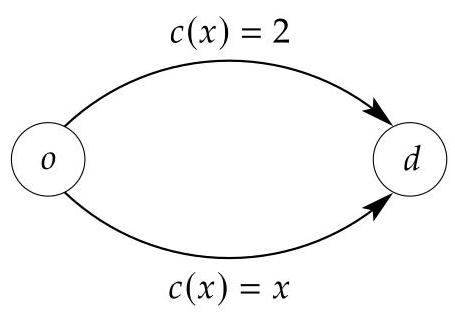
\includegraphics[width=0.3\textwidth]{images/ch02-fig01.jpg}     
    \caption{一个拥塞网络。节点 $o$ 和 $d$ 分别是所有用户的起点和终点；两条平行边的成本 $c(x)$ 取决于相应边上的用户数量 $x$。}
    \label{fig:2.1}
\end{figure}

假设图~\ref{fig:2.1}中的网络有两个用户。他们可能都走上边，也可能一人走一条边，还可能都走下边。如果两人都走上边，则每人的成本都是2；但此时任意一个人单独改走下边，成本就会降为1。因此，这种状态不是均衡，因为至少有一个用户可以单方面改变路线并降低自己的成本。这里需要注意，我们只考虑单个用户的单方面偏离(deviation)。如果两个人同时改走下边，下边会因为 \(x = 2\) 而拥堵，成本又变回2，这并不比两人都走上边更好。

如果两个用户分别走不同的边，则得到一个均衡。走下边的用户当前成本为1，若改走上边，成本会变成2，因此没有改换路线的动机。走上边的用户若改走下边，会使下边的负载从1增加到2，新的成本也为2，对她同样没有好处。因此，没有任何单个用户愿意偏离，这正是均衡的含义。

最后，两人都走下边也是一种均衡。此时两人的成本都是2，而改走上边的成本同样是2，并不会更低。因此，在这个有两个用户的网络中，一共有两类均衡。

这个博弈中的行为称为自私路由(selfish routing)：每个用户只考虑如何选择对自己成本最低的路线。当每个用户都无法靠单方面改换路线获得更低成本时，系统就达到了均衡。

如果用每个用户的平均成本来衡量，自私路由是否总能达到社会最优呢？在这个例子中，一个用户走上边、另一个用户走下边时，二者成本分别为2和1，平均成本为1.5，这显然是社会最优的。相比之下，两个用户都走下边也是均衡，但二者都承担成本2，平均成本更高。
\begin{figure}[ht]
\centering
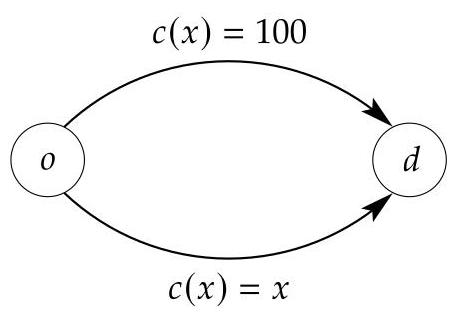
\includegraphics[width=0.3\textwidth]{images/ch02-fig02.jpg}
\caption{与图~\ref{fig:2.1}相同的庇古网络(Pigou network)，但上边的固定成本为 \(c\left( x\right)  = 100\)。这里假设100个用户想从 \(o\) 前往 \(d\)。}
\label{fig:2.2}
\end{figure}

然而，自私路由可能使普通用户的处境比社会最优方案更差。图~\ref{fig:2.2}与图~\ref{fig:2.1}相同，只是上边的固定成本改为100。这个网络称为庇古网络。假设有100个用户都想从 \(o\) 到 \(d\)。不难看出，这个拥塞博弈只有两类均衡：一种是99个用户走下边、1个用户走上边；另一种是100个用户全部走下边。其他状态都不是均衡，因为如果下边至多有98个用户，那么走上边的某个用户改走下边后，成本至多为99，低于原来的100。换句话说，用户会不断涌向下边，直到它的使用成本达到或接近上边的固定成本。

这些均衡的平均成本如下。如果所有用户都走下边，则平均成本为100。如果1个用户走上边、99个用户走下边，则平均成本为99.01，因为
\[
\frac{99}{100}{99} + \frac{1}{100}{100}
 = \frac{99}{100}{99} + \frac{1}{100}\left( {{99} + 1}\right)
 = \frac{{99} + 1}{100}{99} + \frac{1}{100}.
\]

与之相比，如果从 \(o\) 到 \(d\) 的流量在两条边上平均分配，则50个用户走上边，每人承担成本100；50个用户走下边，每人承担成本50。平均成本为
\[
\frac{50}{100}{100} + \frac{50}{100}{50}
 = \frac{1}{2}\left( {{100} + {50}}\right)  = {75}.
\]
下面说明这种50-50的分配确实使平均成本最小。设 \(y\) 个用户走下边，则 \({100} - y\) 个用户走上边。平均成本为
\[
\frac{{100} - y}{100}{100} + \frac{y}{100}y
 = {100} - y + \frac{1}{100}{y}^{2}.
\]
先允许 \(y\) 取任意实数。这个函数对 \(y\) 的导数为 \(- 1 + \frac{2}{100}y\)，仅当 \(y = {50}\) 时为零。由于 \(y = {50}\) 本身就是整数，它也给出了离散情形下的唯一最小值。等价地，
\[
{100} - y + \frac{1}{100}{y}^{2}
 = {100} + \frac{1}{100}{\left( y - {50}\right) }^{2} - \frac{2500}{100},
\]
因此最小值在 \(y = {50}\) 时取得，等于75。

不过要注意，在这个例子中，50-50 的分流绝不是均衡，因为上边的任意用户都会改走下边。用户会不断这样做，直到下边不再更便宜。因此，社会最优的 50-50 分流必须通过某种方式强制实现，例如限制下边的使用，或者通过新的激励机制“改变博弈规则”，比如征收拥堵费。

\section{布雷斯悖论}\label{sec-2.3}

\begin{figure}
\centering
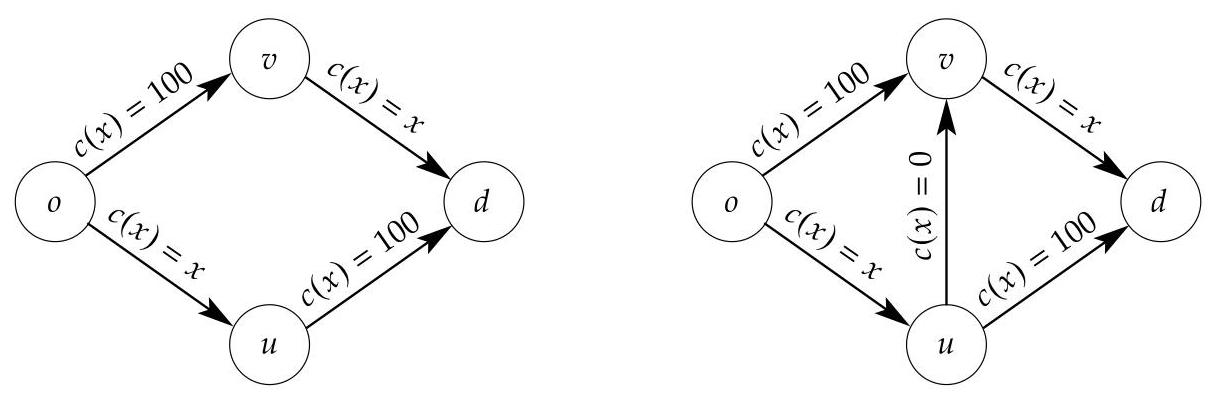
\includegraphics[width=0.9\textwidth]{images/ch02-fig03.jpg}
\caption{布雷斯悖论(Braess paradox)。每条边都有一个成本函数 \(c\left( x\right)\)，其中 \(x\) 是该边上的流量，不同边上的流量可以不同。右侧网络比左侧网络多了一条零成本边 \({uv}\)。对于100个用户，左侧网络的均衡流是最优的；右侧网络虽然容量更大，均衡流反而更差。}
\label{fig:2.3}
\end{figure}


下面讨论一个著名的拥塞博弈，它展示了自私路由可能带来的反直觉结果。图~\ref{fig:2.3}给出了两个拥塞网络。在两个网络中，我们都假设有100个用户想从起点 \(o\) 到终点 \(d\)。先看左侧网络，它只有两条路线：上方路线和下方路线。设 \(y\) 个用户选择经过中间节点 \(u\) 的下方路线，另有 \({100} - y\) 个用户选择经过节点 \(v\) 的上方路线。每条路线都由两条边组成，路线成本就是两条边成本之和。在这种分配下，下方路线的成本为 \(y + {100}\)，上方路线的成本为 \({100} + \left( {{100} - y}\right)\)。在均衡中，两条路线的成本必须相等或几乎相等，否则就会有用户改走更便宜的路线。当 \(y = {50}\) 时，两条路线的成本都等于150，任何用户改走另一条路线只会使那条路线变得更贵。举例来说，若 \(y = {51}\)，则下方路线成本为151，上方路线成本为149；此时下方路线上的一个用户改走上方路线后，新成本为150，反而更低。因此，唯一的均衡是两条路线各有50个用户。也很容易看出，这同时也是该网络的最优流(flow)。

右侧网络比左侧网络多了一条从 \(u\) 到 \(v\) 的边 \({uv}\)。这条边提供了一条“捷径”：用户可以从 \(o\) 出发，依次经过 \(u\)、\(v\)，沿着 \({ou}\)、\({uv}\)、\({vd}\) 到达 \(d\)。设 \(z\) 个用户选择这条新路线。再设 \(y \geq z\)，其中 \(y - z\) 个用户选择从 \(o\) 经 \(u\) 到 \(d\) 的下方路线；这样一来，边 \({ou}\) 上共有 \(y\) 个用户，边 \({ud}\) 上有 \(y - z\) 个用户。剩下 \({100} - y\) 个用户走从 \(o\) 经 \(v\) 到 \(d\) 的上方路线。因此，边 \({ov}\) 的负载为 \({100} - y\)，边 \({vd}\) 的负载为 \({100} - y + z\)。左侧网络可看作边 \({uv}\) 被关闭的情形，也就是 \(z = 0\)。

现在从左侧网络的均衡流出发，即 \(y = {50}\) 且 \(z = 0\)，并假设捷径 \({uv}\) 被打开。此时，从 \(o\) 经捷径到 \(v\) 的成本为50，远低于直接走 \({ov}\) 的成本100；同样，从 \(u\) 经 \(v\) 到 \(d\) 也比走成本为100的边 \({ud}\) 便宜。因此，原来的流不再是均衡。事实上，新的唯一均衡是：边 \({ov}\) 上至多有一个用户，边 \({ud}\) 上至多有一个用户，其余用户都走捷径路线。在最极端的情形下，\(y = z = {100}\)，也就是所有人都走捷径，没有人使用固定成本为100的边 \({ov}\) 和 \({ud}\)。这时，从 \(o\) 到 \(d\) 的总出行成本变为 \({100} + 0 + {100} = {200}\)，而原来只有150。

换个角度看，如果把 \(u\) 和 \(v\) 视为几乎同一个位置，那么成本为零的新边 \({uv}\) 实际上把网络分解成了两个庇古网络，如右图所示。第一个庇古网络从 \(o\) 到目的地 \(v\)，有两条路线：一条是固定成本为100的边 \(ov\)，另一条是先走 \({ou}\) 再走 \({uv}\)，其中成本 \(c\left( x\right)  = x\) 全部来自第一条边 \({ou}\)。第二个庇古网络从 \(u\) 到 \(d\)，同样有两条路线：一条是固定成本为100的边 \({ud}\)，另一条是先走 \({uv}\) 再走 \({vd}\)，其中只有第二条边有成本。与庇古网络一样，在自私路由下，固定成本边 \(ov\) 和 \({ud}\) 基本不会被使用，最多只可能有一个用户使用。

\begin{center}
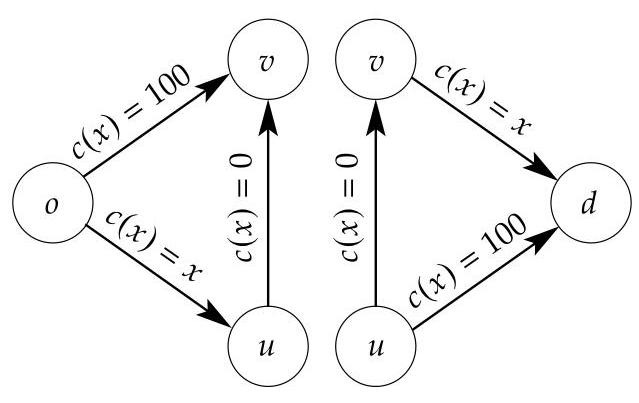
\includegraphics[width=0.5\textwidth]{images/ch02-fig04.jpg}
\end{center}
\hspace*{3em} 

庇古网络说明，自私行为产生的均衡流可能比中央规划下的社会最优流成本更高。图~\ref{fig:2.3}中新增的零成本边 \({uv}\) 则更进一步：它表明给网络增加容量，反而可能让均衡状态下的拥塞更严重，因为新的捷径破坏了原本两条路线之间的平衡。这一现象称为布雷斯悖论(Braess's paradox)，以布雷斯(Braess，1968)命名。

反过来，关闭一条道路有时可能缓解交通拥堵。现实中也能看到类似现象。虽然相关证据大多带有轶事性质，但至少有些城市规划者已经意识到这种可能性。韩国首尔在2002年拆除了清溪川中央河床上的一条大型高速公路，并将其改造成一条长形休闲公园(Hong、Song和Wu，2007，第235页)。这个复杂项目带来的交通改善当然有多重原因，但交通状况确实有所好转。

\section{拥塞博弈的定义}\label{sec-2.4}

本节给出拥塞博弈及其均衡概念的一般定义。一个拥塞网络由以下对象组成:

\begin{itemize}
\item 一个有限的节点(node)集合。
\end{itemize}

\begin{itemize}
\item 一个有限的边(edge)集合 \(E\)。每条边 \(e\) 是一个有序对，记为 \({uv}\)，表示从节点 \(u\) 指向节点 \(v\)，在图中画成从 \(u\) 到 \(v\) 的箭头。我们允许存在平行边(parallel edges)，也就是多条边对应同一个有序对 \({uv}\)，如图~\ref{fig:2.1} 所示。
\end{itemize}

\begin{itemize}
\item 每条边 \(e\) 都配有一个成本函数 \({c}_{e}\)。当边 \(e\) 上有 \(x\) 个用户时，\({c}_{e}\left( x\right)\) 表示每个使用这条边的用户所承担的成本。所有成本函数都弱递增，也就是说，若 \(x \leq  y\)，则 \({c}_{e}\left( x\right)  \leq  {c}_{e}\left( y\right)\)。
\end{itemize}

\begin{itemize}
\item 网络中共有 \(N\) 个用户。每个用户 \(i = 1,\ldots ,N\) 都有一个起点 \({o}_{i}\) 和一个终点 \({d}_{i}\)，二者都是网络中的节点。不同用户的起点和终点可以相同，也可以不同；如果所有用户都共享同一对起终点，我们通常像前面的例子一样将它们记为 \(o\) 和 \(d\)。
\end{itemize}

由节点和边构成的底层结构称为有向图，边有时也称为“弧”。在这样的有向图中，从 \(u\) 到 \(v\) 的路径(path) \(P\) 是一个互不重复的节点序列 \({u}_{0},{u}_{1},\ldots ,{u}_{m}\)，其中 \(m \geq 0\)，\(u = {u}_{0}\)，\(v = {u}_{m}\)，并且对每个 \(0 \leq k < m\)，\({u}_{k}{u}_{k + 1}\) 都是一条边。若 \(e = {u}_{k}{u}_{k + 1}\) 是路径中的一条边，我们记作 \(e \in P\)。注意，同一节点在一条路径中最多出现一次。每个用户 \(i\) 都要从起点 \({o}_{i}\) 到终点 \({d}_{i}\) 选择一条路径，也就是前文所说的路线。

\begin{itemize}
\item 用户 \(i\) 的一个策略是从 \({o}_{i}\) 到 \({d}_{i}\) 的一条路径 \({P}_{i}\) 。
\end{itemize}

\begin{itemize}
\item 给定每个用户 \(i\) 的策略 \({P}_{i}\) 后，边 \(e\) 上的负载或流量(flow)定义为 \({f}_{e} = \left| \left\{  {i \mid  e \in  {P}_{i}}\right\}  \right|\)，也就是所选路径中包含边 \(e\) 的用户数量。在其他用户的策略已定时，用户 \(i\) 选择路径 \({P}_{i}\) 的成本为
\end{itemize}


\setcounter{equation}{0}
\begin{equation}\label{eq:2.1}
\sum_{{e \in  {P}_{i}}}{c}_{e}\left( {f}_{e}\right) .
\end{equation}
由这个网络得到的拥塞博弈，由所有用户的策略集合以及每个策略组合下各用户的成本共同定义。每个用户都独立地试图最小化自己的成本。边 \(e\) 上的流量 \({f}_{e}\) 是使用这条边的用户数，并为每个使用者带来相同的边成本 \({c}_{e}\left( {f}_{e}\right)\)。由于用户选择的路径可能不同，尤其是起点和终点不同时路径必然不同，所以不同用户的总成本也可能不同。

现在考虑用户 \(i\) 将原策略 \({P}_{i}\) 改为另一条路径 \({Q}_{i}\) 时会发生什么。新路径 \({Q}_{i}\) 中有些边原来就在 \({P}_{i}\) 中，这些边构成 \({Q}_{i} \cap {P}_{i}\)；另一些边原来不在 \({P}_{i}\) 中，它们构成 \({Q}_{i} \setminus {P}_{i}\)。显然，\({Q}_{i}\) 中的每条边恰好属于这两类之一。对于 \({Q}_{i} \cap {P}_{i}\) 中的边，流量以及相应成本都保持不变；而对于 \({Q}_{i} \setminus {P}_{i}\) 中的每条边 \(e\)，用户 \(i\) 成为一个新增用户，因此该边的流量从 \({f}_{e}\) 增加到 \({f}_{e}+1\)。如果对用户 \(i\) 的任意替代策略 \({Q}_{i}\)，都有

\begin{equation}\label{eq:2.2}
\sum_{{e \in  {P}_{i}}}{c}_{e}\left( {f}_{e}\right)  \leq \sum _{{e \in  {Q}_{i} \cap  {P}_{i}}}{c}_{e}\left( {f}_{e}\right)  + \sum _{{e \in  {Q}_{i} \setminus  {P}_{i}}}{c}_{e}\left( {{f}_{e} + 1}\right) .
\end{equation}


则称 \({P}_{i}\) 是用户 \(i\) 在其他用户策略 \({P}_{j}\) 已定时的最优反应。这个不等式左边是用户 \(i\) 使用 \({P}_{i}\) 的成本，右边是她偏离到 \({Q}_{i}\) 后的成本。换言之，只要没有任何单方面偏离能带来更低成本，\({P}_{i}\) 就是对其他策略的最优反应。注意，当用户 \(i\) 从 \({P}_{i}\) 改到 \({Q}_{i}\) 时，\({P}_{i}\) 中某些边可能不再被她使用，因此这些边上的流量会减少；这可能有利于那些边上的其他用户，但与用户 \(i\) 自己的新成本无关。最优反应只考虑单个用户的偏离(deviation)。

\begin{definition}\label{def:2.1}如果每个策略都是对其他策略的最优反应，即如果 \eqref{eq:2.2} 对所有 \(i = 1,\ldots ,N\) 都成立，那么所有 \(N\) 个用户的策略 \({P}_{1},\ldots ,{P}_{N}\) 定义了一个均衡。
\end{definition}
前面的例子已经展示了拥塞博弈中的若干均衡。接下来我们证明：这样的均衡总是存在。

\section{拥塞博弈中均衡的存在性}\label{sec-2.5}

下面是本章的核心定理。证明将借助一个势函数(potential function) \(\Phi\)。这个函数把每条边上逐个新增用户所带来的成本累积起来；证明之后我们会解释为什么这样的构造有效。

\begin{theorem}\label{theo:2.2}每个拥塞博弈(从拥塞网络得到)至少有一个均衡。
\end{theorem}
\begin{proof}设 \(N\) 个用户的策略分别为 \({P}_{1},\ldots ,{P}_{N}\)。这些策略在每条边 \(e \in E\) 上诱导出一个流量 \({f}_{e}\)，也就是满足 \(e \in {P}_{i}\) 的用户 \(i\) 的个数。我们将由这些策略诱导出的整体流记为 \(f\)。现在定义流 \(f\) 的函数 \(\Phi \left( f\right)\):

\begin{equation}
\Phi \left( f\right)  = \sum_{{e \in  E}}\left( {{c}_{e}\left( 1\right)  + {c}_{e}\left( 2\right)  + \cdots  + {c}_{e}\left( {f}_{e}\right) }\right)\label{eq:2.3}
\end{equation}

假设用户 \(i\) 将路径从 \({P}_{i}\) 改为 \({Q}_{i}\)，并将由此得到的新流记为 \({f}^{{Q}_{i}}\)。我们将证明

\begin{equation}
\Phi \left( {f}^{{Q}_{i}}\right)  - \Phi \left( f\right)  = \sum_{{e \in  {Q}_{i}}}{c}_{e}\left( {f}_{e}^{{Q}_{i}}\right)  - \sum_{{e \in  {P}_{i}}}{c}_{e}\left( {f}_{e}\right) . \label{eq:2.4}
\end{equation}

根据 \eqref{eq:2.1}，右边正是用户 \(i\) 改用 \({Q}_{i}\) 后的成本与原来使用 \({P}_{i}\) 时的成本之差。她在新流 \({f}^{{Q}_{i}}\) 下的成本，可用原始流 \(f\) 表示为 \eqref{eq:2.2} 右边的形式:

\begin{equation}
\sum_{{e \in  {Q}_{i}}}{c}_{e}\left( {f}_{e}^{{Q}_{i}}\right)  = \sum_{{e \in  {Q}_{i} \cap  {P}_{i}}}{c}_{e}\left( {f}_{e}\right)  + \sum_{{e \in  {Q}_{i} \setminus  {P}_{i}}}{c}_{e}\left( {{f}_{e} + 1}\right) , \label{eq:2.5}
\end{equation}

而她在原始流 \(f\) 下的成本也可类似分解为

\begin{equation}
\sum_{{e \in  {P}_{i}}}{c}_{e}\left( {f}_{e}\right)  = \sum_{{e \in  {P}_{i} \cap  {Q}_{i}}}{c}_{e}\left( {f}_{e}\right)  + \sum_{{e \in  {P}_{i} \setminus  {Q}_{i}}}{c}_{e}\left( {f}_{e}\right) . \label{eq:2.6}
\end{equation}

因此，\eqref{eq:2.4} 的右边可以写成

\begin{equation}
\sum_{{e \in  {Q}_{i}}}{c}_{e}\left( {f}_{e}^{{Q}_{i}}\right)  - \sum_{{e \in  {P}_{i}}}{c}_{e}\left( {f}_{e}\right)  = \sum_{{e \in  {Q}_{i} \setminus  {P}_{i}}}{c}_{e}\left( {{f}_{e} + 1}\right)  - \sum_{{e \in  {P}_{i} \setminus  {Q}_{i}}}{c}_{e}\left( {f}_{e}\right) . \label{eq:2.7}
\end{equation}

由 \eqref{eq:2.3} 的定义可知，\eqref{eq:2.7} 的右侧正好等于 \eqref{eq:2.4} 左侧的 \(\Phi \left( {f}^{{Q}_{i}}\right)  - \Phi \left( f\right)\)。这也是我们这样定义 \(\Phi\) 的原因。具体来说，当用户 \(i\) 从 \({P}_{i}\) 改走 \({Q}_{i}\) 时，对任意新加入的边 \(e \in {Q}_{i} \setminus {P}_{i}\)，该边流量从 \({f}_{e}\) 增加到 \({f}_{e}+1\)，于是 \eqref{eq:2.3} 中相应求和多出一项 \({c}_{e}\left( {{f}_{e} + 1}\right)\)。相反，对任意原来在 \({P}_{i}\) 中、但不再出现在 \({Q}_{i}\) 中的边 \(e \in {P}_{i} \setminus {Q}_{i}\)，流量从 \({f}_{e}\) 减少到 \({f}_{e}-1\)，因此 \eqref{eq:2.3} 中要减去一项 \({c}_{e}\left( {f}_{e}\right)\)。这证明了 \eqref{eq:2.4}。

方程 \eqref{eq:2.4} 表明，任意用户单方面改变策略时，她自身成本的变化正好等于势函数 \(\Phi\) 的变化。现在考虑所有可能的策略组合所诱导出的流 \(f\)，并选取一个使 \(\Phi \left( f\right)\) 达到全局最小值的流。由于策略组合只有有限多个，这样的最小值一定存在。在这个最小点上，任何单个用户改变路线都不可能进一步降低 \(\Phi\)，因此也不可能降低她自己的成本。于是，对应的策略组合就是一个均衡。\end{proof}

定理~\ref{theo:2.2} 证明中引入的函数 \(\Phi\) 值得单独说明。可以这样理解它的定义 \eqref{eq:2.3}。考虑一条边 \(e\)，先假设网络中还没有用户。第一个用户使用边 \(e\) 时，成本为 \(c\left( 1\right)\)；第二个用户加入后，该用户面对的成本为 \(c\left( 2\right)\)；依此类推，直到边上的流量达到 \({f}_{e}\)，最后一个对应的成本为 \(c\left( {f}_{e}\right)\)。不过，\eqref{eq:2.3} 中的和
\[
{c}_{e}\left( 1\right)  + {c}_{e}\left( 2\right)  + \cdots  + {c}_{e}\left( {f}_{e}\right)
\]
并不是边 \(e\) 上所有用户实际支付的总成本。因为当负载为 \({f}_{e}\) 时，每个使用者都承担成本 \(c\left( {f}_{e}\right)\)，所以总成本应为 \({f}_{e} \cdot c\left( {f}_{e}\right)\)，通常大于上面的和。势函数中的这个和，累积的是“依次加入用户”时出现的边成本。

正因为这样定义，\(\Phi\) 才具有关键性质 \eqref{eq:2.4}：任何单个用户改变策略时，该用户成本的变化等于 \(\Phi\) 的变化。一个单一函数 \(\Phi\) 同时捕捉了所有用户的这种单方面变化。具有性质 \eqref{eq:2.4} 的函数称为势函数，具有势函数的博弈称为势博弈(potential game)。由上面的证明可知，任何势博弈都存在均衡，而且可以通过势函数的最小值找到。

性质 \eqref{eq:2.4} 也可以反过来用来寻找均衡。如果某个用户能够通过改变策略降低自身成本，那么同一次改变也会降低势函数 \(\Phi\)。于是可以不断让用户逐个改进自己的策略，使 \(\Phi\) 逐步下降，直到没有用户还能进一步改进为止；此时得到的就是一个均衡。显然，任何均衡都满足这一条件。这样的均衡不一定是势函数的全局最小点，它也可能只是一个“局部”最小点，即单独改变任意一个用户的策略都无法继续降低 \(\Phi\)。在图~\ref{fig:2.1} 的例子中，就存在两个势函数值不同的均衡。

\section{原子流与可拆分流、无政府代价}\label{sec-2.6}

本章提出的有限用户拥塞博弈，只是用自私路由刻画拥塞的众多模型之一。

首先，\eqref{eq:2.1} 中的成本表达式是一种简化。它把用户 \(i\) 看作沿所选路径产生了一个大小为1的“流”，从而对路径上的每一条边都贡献拥塞。这个模型没有刻画时间因素，例如现实中一个用户在某一时刻只能位于一条边上，而不可能同时出现在整条路径上。不过，这种简化并非完全脱离实际，因为用户沿路线移动时，终究会在路径的各个位置与其他用户共同造成拥塞。对互联网路由来说，这种流模型尤其自然：数据包会沿选定路线持续传输并占用带宽。

我们这里研究的模型称为原子流，或不可拆分流。在这个模型中，每个单个用户都完整地选择一条从起点到终点的路径。

与此相对，可拆分流把流量看成由大量“群体”用户组成，其中任意一部分都可以沿不同路径分配。例如，在图~\ref{fig:2.1} 中，从 \(o\) 到 \(d\) 的总流量为2时，可以让0.01单位流量走上边，让1.99单位流量走下边。这仍然不是均衡，因为上边那0.01单位流量中的任意无穷小用户，都可以改走下边来降低自己的成本；单个用户对总流量的影响可以忽略不计。

从某种意义上说，可拆分流更简单，因为它不会出现原子流中那种因“最后一个用户”造成的细微差别。例如在图~\ref{fig:2.2} 中，原子流下底边流量 \(y = {100}\) 和 \(y = {99}\) 都可能对应均衡；而在可拆分流模型中，唯一的均衡流量是 \(y = {100}\)。此时均衡条件更简单：不存在当前成本更低的替代路径即可，而不必像 \eqref{eq:2.2} 中那样考虑切换后某条边的负载从 \({f}_{e}\) 增加到 \({f}_{e}+1\)，从而出现 \({c}_{e}\left( {{f}_{e} + 1}\right)\) 这样的项。在可拆分流模型中，单个用户的规模可以忽略，因此不会造成这种离散增加。

可以证明，可拆分流网络中均衡流的成本是唯一的；不过，达到该成本的均衡流本身可能不唯一，例如两条平行边若具有相同的恒定成本，流量如何分配就可能不确定。对于可拆分流，定理~\ref{theo:2.2} 的证明可以用一个积分形式的势函数 \(\Phi\) 来改写，其中 \({\int }_{0}^{{f}_{e}}{c}_{e}\left( x\right) {dx}\) 取代 \eqref{eq:2.3} 中的求和 \({c}_{e}\left( 1\right)  + {c}_{e}\left( 2\right)  + \cdots  + {c}_{e}\left( {f}_{e}\right)\)；参见拉夫加登(2016 年，第 13.2.2 节)。

在这个背景下，我们还会提到无政府代价(Price of Anarchy)。对一个给定的拥塞网络，它定义为“最差均衡下的平均成本”与“社会最优下的最低平均成本”之比。“无政府”指的是路由博弈中的自私行为，也就是每个用户自行选择对自己最优的路线。在庇古网络中，无政府代价为 \(\frac{100}{75} = \frac{4}{3}\)。对于可拆分流，可以证明：若每条边的成本函数都是仿射函数，即对某些取决于边的非负实数 \(a\) 和 \(b\)，有 \(c\left( x\right)  = {ax} + b\)，那么 \(\frac{4}{3}\) 正是最坏可能情形。(证明可参见 Roughgarden 和 Tardos(2002 年)定理4.5，或 Roughgarden(2016 年)第11章。)换句话说，在仿射成本函数下，自私路由的成本不会比中央规划能够达到的成本高出超过 \(1/3\)。对于不可拆分流，也就是本章主要研究的模型，可以证明仿射成本函数的无政府代价至多为 \(\frac{5}{2}\)(Roughgarden，2016 年，定理12.3)。练习~\ref{exer:2.3} 给出了一个真正达到这一比率的网络，因此在该模型中，\(\frac{5}{2}\) 这个上界是紧的。

\section{延伸阅读}\label{sec-2.7}

本章对定理~\ref{theo:2.2} 的证明参考了 Roughgarden(2016 年)第13章，尤其是其中的定理13.6及其记号。练习~\ref{exer:2.3} 使用的是该书图12.3旋转后的版本，这样更容易看出其对称性。庇古网络最早由庇古(1920 年，第194页)作了定性描述。

布雷斯悖论由布雷斯(1968 年)提出。练习~\ref{exer:2.2} 讨论的是布雷斯原文中实际使用的网络。Hong、Song 和 Wu(2007 年)在讨论清溪川城市再生项目时并未提到布雷斯悖论，但他们在第235页给出了一些很好的“前后”对比图，并且为本书增添了一点风水色彩。

利用势函数 \(\Phi\) 证明原子自私路由中均衡存在性的思想，最早由罗森塔尔(Rosenthal，1973 年)提出。在更一般的博弈中，那些可以借助势函数寻找均衡的博弈，被蒙德勒和夏普利(Monderer\& Shapley，1996)系统研究，并称为势博弈。

可拆分流模型由沃德罗普(Wardrop，1952 年)提出，其均衡通常称为用户均衡(Wardrop equilibrium)。

\section{第2章练习}

\begin{exercise}\label{exer:2.1}考虑下面的拥塞网络。起点为 \(o\)，终点为 \(d\)，中间节点为 \(v\)。共有十个个体用户想从 \(o\) 前往 \(d\)。

\begin{center}
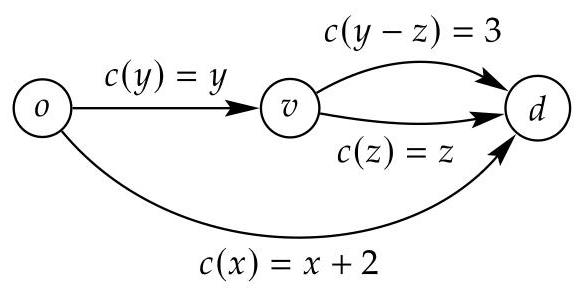
\includegraphics[width=0.4\textwidth]{images/ch02-fig05.jpg}
\end{center}
\hspace*{3em} 

如图所示，若底部直达边上有 \(x\) 个用户，则该边成本为 \(c\left( x\right)  = x + 2\)，其中 \(x + y = {10}\)。从 \(o\) 到 \(v\) 的边成本为 \(c\left( y\right)  = y\)。从 \(v\) 到 \(d\) 的上边成本恒为3；从 \(v\) 到 \(d\) 的下边若有 \(z\) 个用户使用，则成本为 \(c\left( z\right)  = z\)，其中 \(0 \leq  z \leq  y\)。

(a) 求出这个拥塞博弈的所有均衡，并给出各均衡下每个用户的最终平均成本。注意 \(x,y,z\) 都是整数。[提示:先判断均衡中 \(z\) 可能取哪些值。]

(b) 仍考虑同一个网络，但现在从 \(o\) 到 \(d\) 的总流量为10，且 \(x,y,z\) 可以取分数值，也就是流量可拆分。求出此时的均衡，并将其平均成本与(a)中的均衡成本比较。
\end{exercise}
\begin{exercise}\label{exer:2.2}考虑下面两个拥塞网络。图中标出了各边关于其流量 \(x\) 的成本函数；例如，\({50} + x\) 是 \(c\left( x\right)  = {50} + x\) 的简写。注意，不同边上的流量 \(x\) 可能不同，这取决于用户选择的路线。

\begin{center}
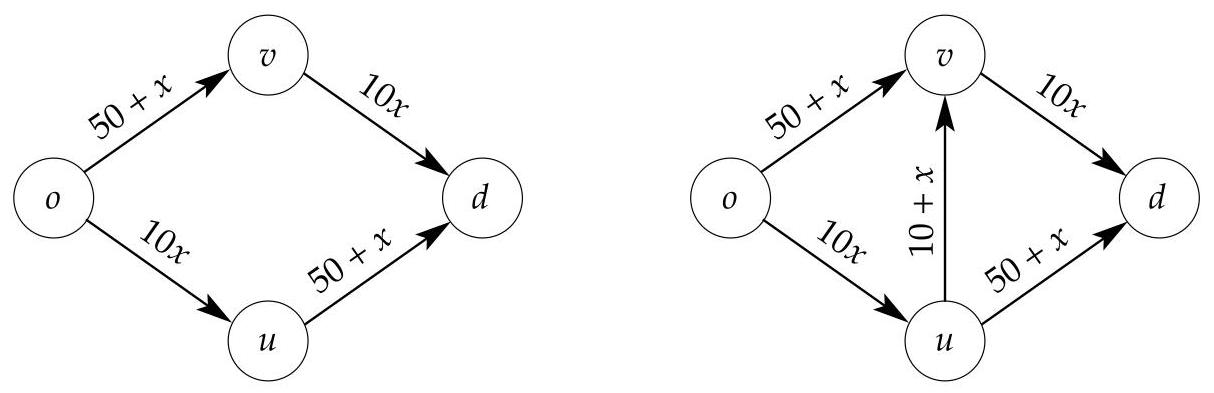
\includegraphics[width=0.9\textwidth]{images/ch02-fig06.jpg}
\end{center}
\hspace*{3em} 

假设共有六个用户想从 \(o\) 前往 \(d\)。

(a) 求出左侧网络中的均衡流。

(b) 在右侧网络中，从(a)得到的均衡流出发，每次只让一个用户改进自己的路线，直到达到一个均衡流。比较两个网络中的均衡成本。
\end{exercise}
\begin{exercise}\label{exer:2.3}
考虑下面这个有三个节点的拥塞网络。如图所示，除边 \({vu}\) 和 \({wu}\) 外，每条边在流量(即用户数量)为 \(x\) 时的成本均为 \(c\left( x\right)  = x\)；而在边 \({vu}\) 和 \({wu}\) 上，成本为 \(c\left( x\right)  = 0\)。右侧表格给出了四个用户 \(i = 1,2,3,4\) 的起点 \({o}_{i}\) 和终点 \({d}_{i}\)。在这个网络中，每个用户从自己的起点到终点都有两条可选路线。

\begin{center}
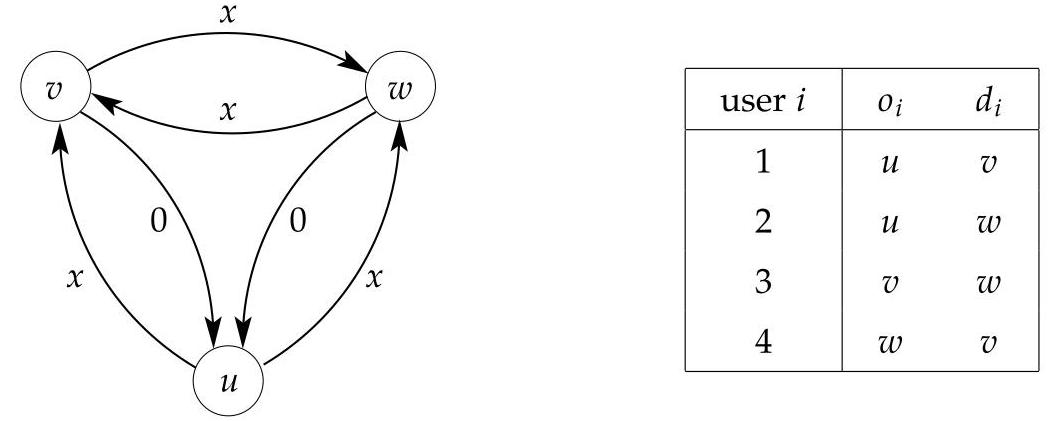
\includegraphics[width=0.8\textwidth]{images/ch02-fig07.jpg}
\end{center}
\hspace*{3em} 

求出这个拥塞博弈的两个均衡：一个低成本均衡和一个高成本均衡。分别说明为什么它们满足均衡条件，并比较这两个均衡的成本。社会最优流是什么？它可以不是均衡。

\end{exercise}